\documentclass[twocolumn]{article}
\usepackage{amsmath}
\usepackage{amssymb}
\usepackage{graphicx}

\begin{document}

\section*{Numbers}

\subsection*{Types of Numbers:}

\begin{itemize}
\item Natural Numbers: $\mathbb{N} = \{1,2,3, \ldots\}$
\item Whole Numbers: $\mathbb{N} \cup \{0\} =\{0,1,2,3, \ldots\}$
\item Integers: $\mathbb{Z} =\{\ldots,-2,-1,0,1,2, \ldots\}$
\item Rational Numbers: $\mathbb{Q} = \left\{\frac{a}{b} \ : \  a, b \in \mathbb{Z} \ , \ b \neq 0 \right\}$. Rational Numbers comprise of fractions (includes all proper and improper fractions and mixed numbers). All terminating decimals (eg, $10.87$) and recurring decimals (eg, $0.3\dot{7}\dot{1} = 0.3717171\ldots$) are rational numbers because these can all be expressed as fractions. All integers are rational numbers.
\item Irrational Numbers: numbers that cannot be expressed in the form $\frac{a}{b}$, where $a$ and $b$ are integers and $b \neq 0$. Eg. $\pi$, $\sqrt{2}$, $\sqrt{5}$, $-4\sqrt{7}$, $e$, $2.75e$, etc. Irrational numbers are non-recurring decimals. Any non-zero rational number multiplied to an irrational number results in an irrational number. For example, $-\frac{3}{4}\pi$ is irrational.
\item Perfect Squares: $\{1,4,9,16,25, \ldots\}$
\item Perfect Cubes: $\{1,8,27,64, \ldots\}$
\item Prime Numbers: Positive integers at least 2 whose only positive divisors are 1 and itself. $\{2,3,5,7,11,13,17,19,23, \ldots\}$
\end{itemize}

\subsection*{Equality and Inequality Symbols}

\begin{tabular}{|c|l|l|}
	\hline Symbol & \multicolumn{1}{|c|}{ Meaning } & \multicolumn{1}{|c|}{ Example } \\
	\hline$=$ & is equal to & $0.1=\frac{1}{10}$ \\
	\hline$\neq$ & is not equal to & $0.11 \neq \frac{1}{10}$ \\
	\hline$>$ & is greater than & $0.1>0.01$ \\
	\hline$\geqslant$ & is greater than or equal to & $a \geqslant 5$ \\
	\hline$<$ & is less than & $0.05<5$ \\
	\hline$\leqslant$ & is less than or equal to & $b \leqslant 5$ \\
	\hline
\end{tabular}

\subsection*{Prime Factorization, HCF, LCM} 

\begin{itemize}
\item Example of prime factorization:

\begin{tabular}{r|c}
	2 & 4356 \\
	\cline { 2 - 2 } 2 & 2178 \\
	\cline { 2 - 2 } 3 & 1089 \\
	\cline { 2 - 2 } 3 & 363 \\
	\cline { 2 - 2 } 11 & 121 \\
	\cline { 2 - 2 } & 11 \\
	\hline 
\end{tabular}

Hence $4356=2^2 \times 3^2 \times 11^2$ (in index notation).

\item Example of HCF and LCM using prime factorization:

$
\begin{aligned}
	& 4800=2^6 \times 3 \times 5^2 \\
	& 5544=2^3 \times 3^2 \times 7 \times 11
\end{aligned}
$

$\mathrm{HCF}=2^3 \times 3$

[take common prime factors and lowest power of each]

$\mathrm{LCM}=2^6 \times 3^2 \times 5^2 \times 7 \times 11$

[take all prime factors and highest power of each]

\item Examples of square roots and cube roots using prime factorization:

$\begin{aligned} 54756 & =2^2 \times 3^4 \times 13^2 \\ \sqrt{54756} & =2 \times 3^2 \times 13 = 234\end{aligned}$

$\begin{aligned} 1728 & =2^6 \times 3^3 \\ \sqrt[3]{1728} & =2^2 \times 3 = 12\end{aligned}$
\end{itemize}

\subsection*{Approximation}

\subsubsection*{Significant Figures}

\noindent
Rules of identifying number of significant digits:

\begin{enumerate} 
\item All non-zero digits are significant.
\item Zeros between non-zero digits are significant. 

Eg. 302 (3 sf)

Eg. 10.2301 (6 sf)

\item In a whole number, zeros after the last nonzero digit may or may not be significant. It depends on the estimation being made.

Eg.

$
\begin{aligned}
	& 7436000=7000000 \ (1 \ \mathrm{sf}) \\
	& 7436000=7400000 \ (2 \ \mathrm{sf}) \\
	& 7436000=7440000 \ (3 \ \mathrm{sf}) \\
	& 7436000=7436000 \ (4 \ \mathrm{sf}) \\
	& 7436000=7436000 \ (5 \ \mathrm{sf}) \\
	& 7436000=7436000 \ (6 \ \mathrm{sf}) \\
\end{aligned}
$

\item In a decimal number, zeros before the $1^{\text{st}}$ non-zero digit are not significant.

Eg. $0.004 \ (1 \ \mathrm{sf})$

Eg. $0.07008 \ (4 \ \mathrm{sf})$

\item In a decimal number, zeros after the last non-zero digit are significant.

Eg. $6.40 \ (3 \ \mathrm{sf})$

Eg. $12.000 \ (5 \ \mathrm{sf})$

Eg. $20300.000 \ (8 \ \mathrm{sf})$

Eg. $0.0700800 \ (6 \ \mathrm{sf})$
\end{enumerate} 

\subsubsection*{Decimal Place Rounding}

\noindent 
Examples:

\noindent
$
\begin{aligned}
	& 0.7374=0.74 \ (2 \ \mathrm{dp}) \\
	& 58.301=58.30 \ (2 \ \mathrm{dp}) \\
	& 207.6296=207.630 \ (3 \ \mathrm{dp}) \\
	& 207.6296=207.63 \ (2 \ \mathrm{dp}) \\
    & 207.977=208.0 \ (1 \ \mathrm{dp}) \\
    & 207.977=207.98 \ (2 \ \mathrm{dp}) \\
    & 18.997=19.00 \ (2 \ \mathrm{dp})
\end{aligned}
$

\subsection*{Standard Form}

\noindent
$\pm A \times 10^n$, where $1 \leq A < 10$ and $n$ is an integer.

\bigskip 

\noindent
Examples:

\noindent
$
\begin{aligned}
	& 1350000=1.35 \times 10^6 \\
	& 0.000375=3.75 \times 10^{-4}
\end{aligned}
$

\subsection*{Common Prefixes}

\begin{tabular}{|l|l|l|l|}
	\hline $10^{12}$ & trillion & tera & $\mathrm{T}$ \\
	\hline $10^9$ & billion & giga & $\mathrm{G}$ \\
	\hline $10^6$ & million & mega & $\mathrm{M}$ \\
	\hline $10^3$ & thousand & kilo & $\mathrm{k}$ \\
	\hline $10^{-3}$ & thousandth & milli & $\mathrm{m}$ \\
	\hline $10^{-6}$ & millionth & micro & $\mu$ \\
	\hline $10^{-9}$ & billionth & nano & $\mathrm{n}$ \\
	\hline $10^{-12}$ & trillionth & pico & $\mathrm{p}$ \\
	\hline
\end{tabular}

\subsection*{Indices}

\noindent 
Rules of Indices:

\noindent 
$\begin{gathered} a^0=1 \\ a^m \times a^n=a^{m+n} \\ a^m \div a^n=a^{m-n} \\ (a b)^n=a^n b^n \\ \left(\frac{a}{b}\right)^n=\frac{a^n}{b^n} \\ \left(a^n\right)^m=a^{n m} \\ a^{-n}=\frac{1}{a^n} \\ \left(\frac{a}{b}\right)^{-n}=\left(\frac{b}{a}\right)^n=\frac{b^n}{a^n} \\  a^{\frac{1}{n}}=\sqrt[n]{a} \\ a^{\frac{m}{n}}=\sqrt[n]{a^m}=(\sqrt[n]{a})^m\end{gathered}$

\noindent
Caution:

\noindent
1. For indices (powers) that are not integers, then the above rules of indices hold only for $a,b \geq 0$, or only for $a,b > 0$ if some of the indices are negative or there is division by either $a$ or $b$. The rule $a^0=1$ holds only for non-zero values of $a$.

\noindent
2. $\sqrt{(-8)^2} = \sqrt{64} = 8$, NOT $-8$.

\noindent
3. $\sqrt[3]{-27} = -3$.

\bigskip 

\noindent 
Equalities of Indices:

\noindent 
1. If $a^m=a^{\prime \prime}$, then $m=n$.

\noindent 
2. If $a^m=b^m$, then $a=b$.

\subsection*{Direct and Inverse Proportion}

\noindent 
If $y$ is directly proportional to $x$, then $y=k x$, where $k$ is a constant and $k \neq 0$. The ratios $\frac{x}{y}$ and $\frac{y}{x}$ are constant. Furthermore, the graph on $y$ against $x$ (or of $x$ against $y$) is a straight line through the origin.

\noindent
Graph showing that $y$ is directly proportional to  $x$:

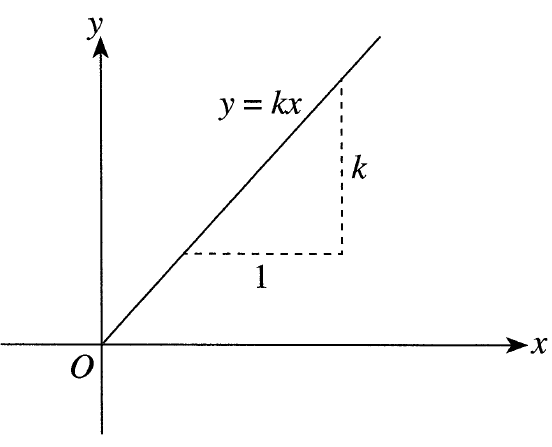
\includegraphics[width=0.4\textwidth]{01.png}

\bigskip 

\noindent 
If $y$ is inversely proportional to $x$, then $y=\frac{k}{x}$, where $k$ is a constant and $k \neq 0$. The product $xy$ is constant. 

\noindent
Graph showing that $y$ is inversely proportional to  $x$:

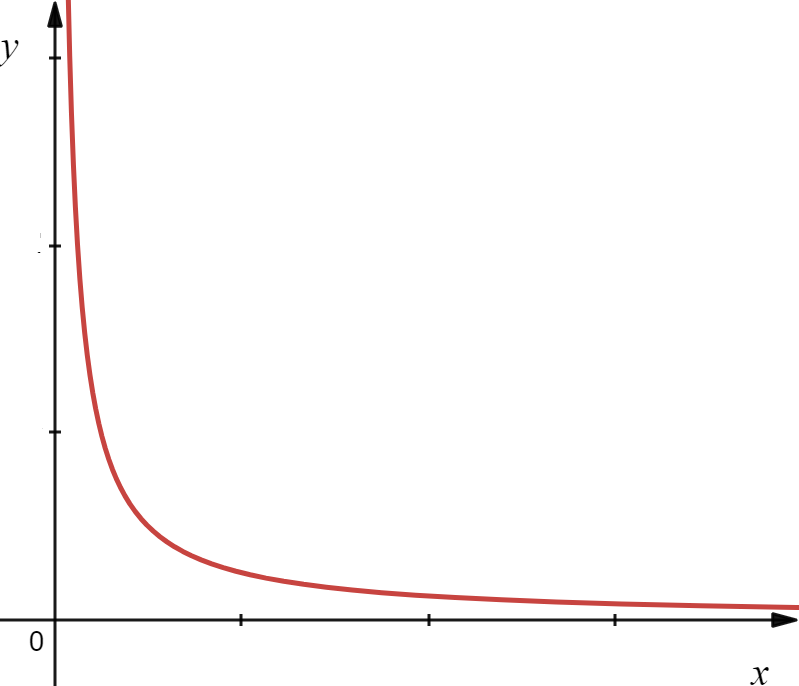
\includegraphics[width=0.4\textwidth]{02.png}

\subsection*{Map Scales}

\begin{itemize}  

\item Linear scale:

$1: n$ means $1$ unit length on map represents $n$ units length on ground.

Eg. $1 : 5000$ means

$1 \mathrm{~cm}$ represents $5000 \mathrm{~cm}$

which implies $1 \mathrm{~cm}$ represents $50 \mathrm{~m}$

which implies $1 \mathrm{~cm}$ represents $0.05 \mathrm{~km}$

\item Representative Fraction (RF):

If the linear scale is $1:n$, the RF is expressed as $\frac{1}{n}$.

Eg, if 3 cm represents 6 m, then RF is $\frac{1}{200}$.

\item Area Scale:

If linear scale is $1:200000$, then it means 

$1 \mathrm{~cm}$ represents $200000 \mathrm{~cm}$

which implies  $1 \mathrm{~cm}$ represents $0.2 \mathrm{~km}$

which implies $1^2 \mathrm{~cm}^2$ represents $(0.2)^2 \mathrm{~km}^2$

which implies $1 \mathrm{~cm}^2$ represents $0.04 \mathrm{~km}^2$
\end{itemize} 

\subsection*{Percentage, Ratio, Rate}

\begin{itemize}  

\item To express a percentage as a fraction or decimal, divide by $100$:

$
x \%=\frac{x}{100}
$

Eg, $23.5 \% = \frac{23.5}{100} = \frac{235}{1000} = \frac{47}{200}$

Eg, $401 \% = \frac{401}{100} = 4.01$

\item To express any number as a percentage, multiply it by $100 \%$.

Eg, $0.165 = 0.165 \times 100 \% = 16.5 \%$.

\item Expressing a quantity $A$ as a percentage of a quantity $B$

$
\frac{A}{B} \times 100 \%
$

Eg, Express $63.7$ as a percentage of $98$. 

Answer: $\frac{63.7}{98} \times 100\% = 65 \%$

In words, we say that $63.7$ is $65 \%$ of $98$. 

\item Increase or decrease a quantity by a given percentage:

Eg, Increase $45$ by $2.4 \%$:

Answer: $45 \times \left(1+\frac{2.4}{100}\right) = 45 \times 1.024 = 46.08$  

Eg, Decrease $45$ by $90 \%$:

Answer: $45 \times \left(1-\frac{90}{100}\right) = 45 \times 0.1 = 4.5$

\item Percentage Increase and Percentage Decrease:

When a quantity increases, the percentage increase is

$\frac{\text{final value} \ - \ \text{initial value}}{\text{initial value}} \times 100\%$

When a quantity dereases, the percentage decrease is

$\frac{\text{initial (bigger) value} \ - \ \text{final (smaller) value}}{\text{initial value}} \times 100\%$

Percentage increase will always be $> 0$ if the quantity has increased.

Percentage decrease will always be $> 0$ if the quantity has decreased.

Percentage change is

$\frac{\text{final value} \ - \ \text{initial value}}{\text{initial value}} \times 100\%$

regardless of whether the quantity has increased or decreased. Percentage change can be either positive or negative depending on whether the quantity has increased or decreased.

\end{itemize}  


\end{document}